
\chapter{Properties of Motors and Muscles}
\label{sec:PropertiesOfMotorsAndMuscles}

Unfortunately, current technologies do not allow us to replicate the properties of muscles exactly. Muscles are strong and light, and can fit into extremely small spaces while still being able to deliver tremendous force. The two most robust forms of actuators in use today on legged robots are hydraulics and electric motors. Hydraulics are powerful, but they are extremely inefficient and can leak oil. Electric motors are far more efficient consumers of energy, and thus will be the main focus of actuation options in this book. This chapter starts with an introduction to the properties of electric motors and a discussion of the power they use. The section on electric motors is followed by an introduction to human locomotive muscle properties, and how these muscles compare to electric motors.

\section{Introduction to Motors} % (notes page 3-7)
\label{IntroductionToMotors}
\index{motors}

Generally speaking, using stored electricity to power electric actuators is extremely efficient. One Joule of electric energy stored in a battery or capacitor will deliver almost one Joule of energy to an electric motor paired with the storage device. Compare this to gasoline, where the amount of energy stored in chemical bonds is approximately four times the amount of thermal energy that results from combustion.

A basic configuration of an electric motor and a power supply is shown in figure \ref{fig:PowerSupplyAndMotor}. The voltage and current associated with the power supply are $V$ and $I$, respectively. The angular speed and torque provided by the motor are $\omega$ and $T$, respectively.

% FIGURE
\begin{figure}[h]		% h="here" t="top" b="bottom" p="separate page"
\begin{centering}
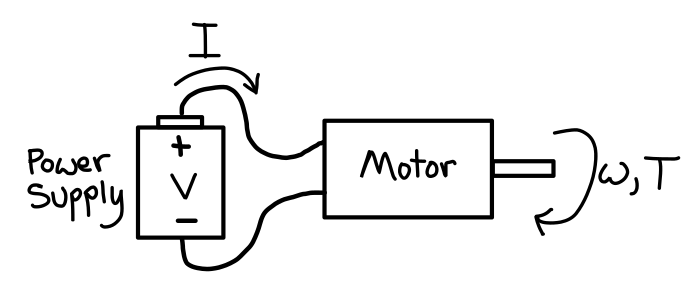
\includegraphics[width=0.5\textwidth]{Figures/PowerSupplyAndMotor}\par
\end{centering}
\caption[Diagram: Power Supply and Electric Motor]{Power supply and electric motor. The power supply provides $I$ Amperes of current at a potential difference of $V$ Volts. This creates $T$ Newton-meters of torque and spins the motor at $\omega$ radians per second.}
\label{fig:PowerSupplyAndMotor}
\end{figure}
%

We are interested in the relationships between $I$, $V$, $\omega$, and $T$. Given that we have four variables, if we choose one of them to control, we will then be left with three equations that govern the other variables.

\subsection*{Power}
\label{sec:Power}

The power consumed and developed by the configuration shown in figure \ref{fig:PowerSupplyAndMotor} is described by the following equations:

\begin{equation}
P_{i}=P_{in} = \mbox{electric power into motor}= IV
\label{eq:PowerIn}
\end{equation}

\begin{equation}
P_{o}=P_{out} = \mbox{power motor exerts on environment} = T\omega
\label{eq:PowerOut}
\end{equation}

The fundamental restriction on electric motors is that there is always positive dissipation due to heat loss, and input power from the battery is greater than power output by the motor. This holds true for many types of actuation systems, as it is nearly impossible to build a completely lossless machine or system. Figure \ref{fig:IdealPowerPlotSketch} demonstrates this fundamental restriction.

% FIGURE
\begin{figure}[h]		% h="here" t="top" b="bottom" p="separate page"
\begin{centering}
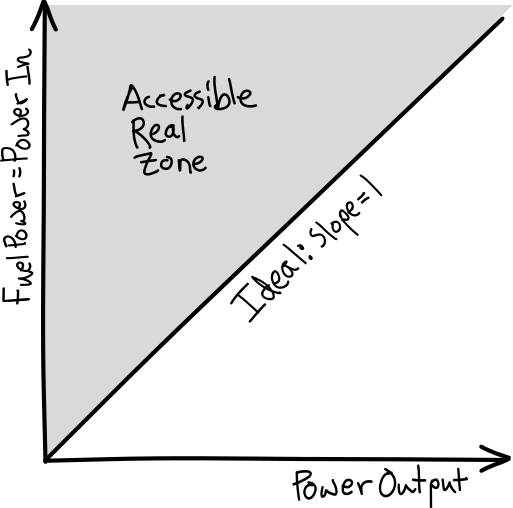
\includegraphics[width=0.5\textwidth]{Figures/IdealPowerPlotSketch}\par
\end{centering}
\caption[Plot: Power Conservation]{Fuel power input to a system vs. the power output by the system. An ideal system would produce as much power in the form of mechanical work as it consumes in chemical energy from fuel. The shaded area of this plot represents the performance levels attainable by real systems.}
\label{fig:IdealPowerPlotSketch}
\end{figure}
\index{power}

Imagine for one instant in time, $\omega$ is fixed. This leaves three variables: $T$, $V$, and $I$ to control in some way. If $V$ and $I$ are controlled, equations \ref{eq:PowerIn} and \ref{eq:PowerOut} become the following two equations:

\begin{equation}
IV = T\omega + I^2R
\label{eq:EnergyConservation}
\end{equation}

where the $I^2R$ term represents the internal resistance of the motor. Additionally, we can quantify the motor torque:

\begin{equation}
T = kI
\label{eq:MotorTorque}
\end{equation}

where $k$ represents the motor torque constant, which has units of [Nm/Amp]. Substitution of equation \ref{eq:MotorTorque} into equation \ref{eq:EnergyConservation}, gives the motor voltage law:
\begin{equation}
V = k\omega + IR
\label{eq:MotorVoltage}
\end{equation}

We think of equations \ref{eq:MotorTorque} and \ref{eq:MotorVoltage} as describing a motor that is controlled by a given voltage. So if given a voltage, say 9 volts, we would like to eliminate $I$ from these two equations so that we can see how the machine behaves. Manipulation yields:

\begin{equation}
V = k\omega + \frac{T}{k}R
\label{eq:MotorVoltage2}
\end{equation}

\begin{equation}
T = \frac{k}{R}V - \frac{k^2}{R}\omega
\label{eq:MotorTorque2}
\end{equation}

Figure \ref{fig:MotorTorqueCurveSketch} shows what equation \ref{eq:MotorTorque2} looks like:

% FIGURE
\begin{figure}[h]		% h="here" t="top" b="bottom" p="separate page"
\begin{centering}
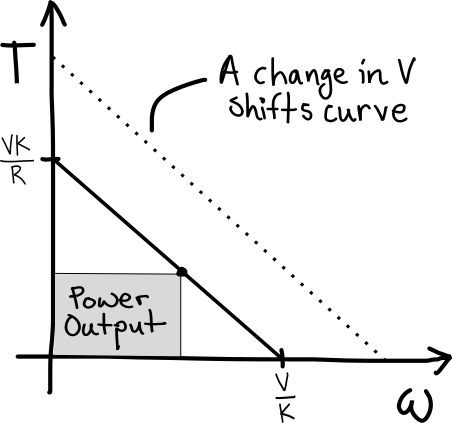
\includegraphics[width=0.4\textwidth]{Figures/MotorTorqueCurveSketch}\par
\end{centering}
\caption[Plot: Torque vs. Angular Speed for an Electric Motor]{Torque vs. angular speed for an electric motor. The relationship is linear, described by $T = \frac{k}{R}V - \frac{k^2}{R}\omega$ (equation \ref{eq:MotorTorque2}). Notice that $\frac{Vk}{R}$, the intersection of the curve and the torque axis, is directly proportional to $V$. The power developed by the motor, $T\omega$, is the area of the shaded rectangle for a given operating point.}
\label{fig:MotorTorqueCurveSketch}
\end{figure}
%

An important quantity to solve for is the free spinning angular rate, $\omega_{f}$:

\begin{equation}
\omega_{f} = \frac{1}{k}V
\label{eq:FreeSpinningOmega}
\end{equation}

and with manipulation, we can find the value of the motor torque constant in terms of $\omega_{f}$:

\begin{equation}
k = \frac{V}{\omega_{f}}
\label{eq:MotorTorqueConstant}
\end{equation}

where $k$ has units of $[\frac{V}{rad/s}]$.

It's useful here to demonstrate the energy used by the motor:

\begin{equation}
P_{i} = VI = V\frac{T}{k} = \frac{V}{k}\left(\frac{k}{R}V - \frac{k^2}{R}\omega\right)
\label{eq:MotorPowerUse}
\end{equation}

equation \ref{eq:MotorPowerUse} describes the power consumed by the motor, which is equal to the power supplied by the battery. This power is called the input power. This power relationship is shown in figure \ref{fig:PowerVsOmega} as a straight line, where the curved line is the output power, $P_{o}$:

\begin{equation}
P_{o} = T\omega= \left(\frac{k}{R}V - \frac{k^2}{R}\omega\right)\omega
\label{eq:MotorPowerOutput}
\end{equation}

%% FIGURE
%\begin{figure}[h]		% h="here" t="top" b="bottom" p="separate page"
%\begin{centering}
%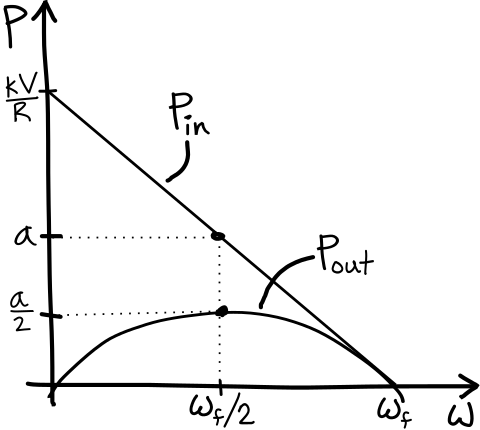
\includegraphics[width=0.4\textwidth]{Figures/PowerVsOmega}\par
%\end{centering}
%\caption[Plot: Output Motor Power vs. $\omega$]{Output motor power versus rotational speed, $\omega$. This plot shows equations \ref{eq:MotorPowerOutput} and \ref{eq:MotorPowerUse} on the same axis. The rotational speed that produces the greatest power output is half of the free spinning rotational speed of the motor. The required power drawn from the battery at this speed is twice the developed power, as indicated by the points labeled $a$ and $a/2$ on the P axis.}
%\label{fig:PowerVsOmega}
%\end{figure}
%%

Given the input and output power, we can calculate the motor efficiency:

\begin{equation}
\mbox{efficiency} = \frac{P_{o}}{P_{i}}
\label{eq:MotorEfficiency}
\end{equation}

At peak power, $\omega = \frac{\omega_{f}}{2}$ and the efficiency therefore equals 50\%. The peak efficiency is close to 1 when $\omega$ approaches $\omega_{f}$. The efficiency is shown in figure \ref{fig:MotorEfficiency}.

%% FIGURE
%\begin{figure}[h]		% h="here" t="top" b="bottom" p="separate page"
%\begin{centering}
%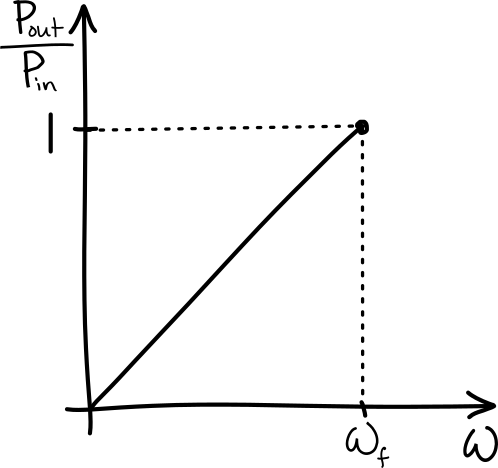
\includegraphics[width=0.3\textwidth]{Figures/MotorEfficiency}\par
%\end{centering}
%\caption[Plot: Electric Motor Power and Efficiency vs. $\omega$.]{Electric motor efficiency versus $\omega$. An electric motor is most efficient when it is allowed to spin at its free spinning rotational speed. However, as shown in figure \ref{fig:PowerVsOmega}, the motor produces no power when it spins at its free spinning rotational speed.}
%\label{fig:MotorEfficiency}
%\end{figure}
%%

% FIGURE
\begin{figure}[h]		% h="here" t="top" b="bottom" p="separate page"
\begin{center}
 \subfloat[]{\label{fig:PowerVsOmega}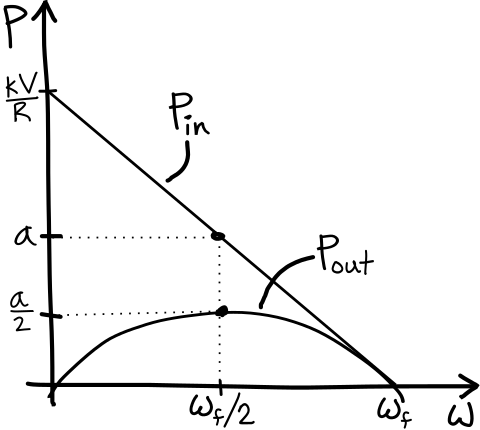
\includegraphics[width=0.48\textwidth]{Figures/PowerVsOmega}} \hspace{0.05\textwidth}%
 \subfloat[]{\label{fig:MotorEfficiency}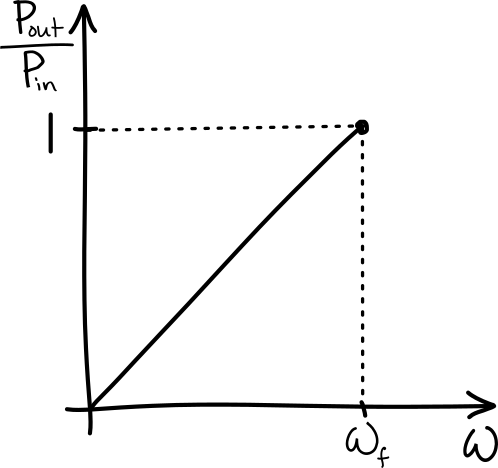
\includegraphics[width=0.43\textwidth]{Figures/MotorEfficiency}}
\end{center}
\caption[Plot: Electric Motor Power and Efficiency vs. $\omega$.] {(a) Output motor power vs. rotational speed, $\omega$. This plot shows equations \ref{eq:MotorPowerOutput} and \ref{eq:MotorPowerUse} on the same axis. The rotational speed that produces the greatest power output is half of the free spinning rotational speed of the motor. The required power drawn from the battery at this speed is twice the developed power, as indicated by the points labeled $a$ and $a/2$ on the P axis.  (b) Electric motor efficiency vs. $\omega$. An electric motor is most efficient when it is allowed to spin at its free spinning rotational speed. However, as shown in figure \ref{fig:PowerVsOmega}, the motor produces no power when it spins at its free spinning rotational speed.}
\label{fig:MotorPowerAndEfficiency}
\end{figure}
%

So now given a basic motor model, we can compare plots of various quantities, as in figure \ref{fig:FourMotorCurves}.

% FIGURE
\begin{figure}[h]		% h="here" t="top" b="bottom" p="separate page"
\begin{centering}
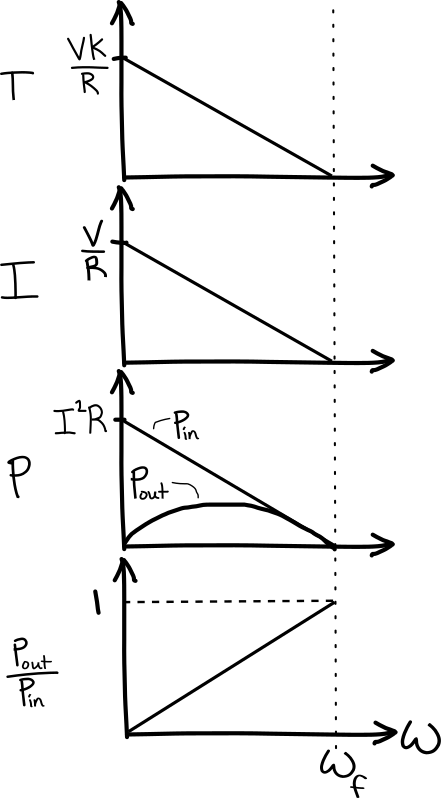
\includegraphics[width=0.35\textwidth]{Figures/FourMotorCurves}\par
\end{centering}
\caption[Plot: A Comparison of Four Motor Curves vs. $\omega$]{A comparison of motor torque, current, power, and efficiency. The torque, $T$, is a linear function of $\omega$, as is the current, $I$. The current function is simply the torque function scaled by $k$. The bottom two plots are the power and efficiency curves from figure \ref{fig:MotorPowerAndEfficiency}, shown again to emphasize that the motor produces no torque and draws no current at its free spinning rotational speed.}
\label{fig:FourMotorCurves}
\end{figure}
%

Key points to remember regarding efficiency: Running a motor slowly is not very efficient. Running a motor near free speed is very efficient. So given any motor, we can increase $V$ arbitrarily and get any power at any efficiency we choose. Sounds great, but here's the catch: as we increase $V$ at a fixed efficiency, we also inadvertently must change $\omega$, which may not be desirable. What's the solution? Gearboxes.

A gearbox is a passive box that yields $P_{in}=P_{out}$:

\begin{equation}
T_{in}\omega_{in} = T_{out}\omega_{out}
\label{eq:GearboxExample}
\end{equation}

% FIGURE
\begin{figure}[h]		% h="here" t="top" b="bottom" p="separate page"
\begin{centering}
 \subfloat[]{\label{fig:GearboxExample}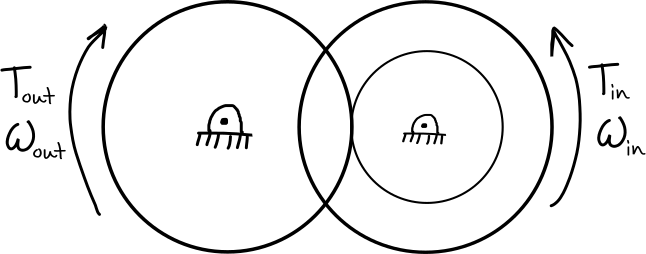
\includegraphics[width=0.5\textwidth]{Figures/GearboxExample}} \hspace{0.1\textwidth}%
 \subfloat[]{\label{fig:PulleyExample}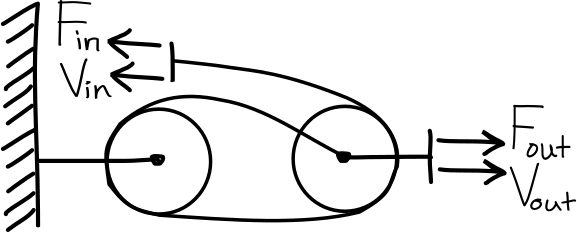
\includegraphics[width=0.4\textwidth]{Figures/PulleyExample}}
\end{centering}
\caption[Diagram: Force Amplification with Gearbox and Pulley Systems]{(a) A simple gear system. In this case, the input torque $T_{in}$ is amplified, while the input rotational speed $\omega_{in}$ is reduced ($T_{out}>T_{in}$ and $\omega_{out}<\omega_{in}$). (b) A simple pulley system. In this case, the output force is amplified, while the output velocity is reduced ($F_{out}>F_{in}$ and $V_{out}<V_{in}$). For both systems, power is conserved.}
\label{fig:GearboxAndPulleyExample}
\end{figure}
%

It's important to realize one drawback of gearboxes. As we amplify the force, we reduce velocity. This is best illustrated with a pulley example:

\begin{equation}
F_{in}v_{in} = F_{out}v_{out}
\label{eq:PulleyExample}
\end{equation}

One of the key problems in robotics is how to appropriately size a gearbox. The key equations for this problem are shown in equation \ref{eq:MotorAndGearbox}.

\begin{align}
T_{out} &=GT_{in} \notag \\
\omega_{out} &=\omega_{in}/G \notag \\
T_{in}\omega_{in}&=T_{out}\omega_{out}
\label{eq:MotorAndGearbox}
\end{align}

These equations  \ref{eq:MotorAndGearbox} neglect the presence of friction.

% FIGURE
\begin{figure}[h]		% h="here" t="top" b="bottom" p="separate page"
\begin{centering}
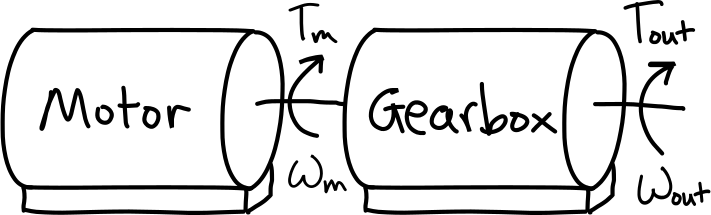
\includegraphics[width=0.5\textwidth]{Figures/MotorAndGearbox}\par
\end{centering}
\caption[Diagram: Motor Connected to a Gearbox]{A motor connected to a gearbox. The motor develops a torque $T_{m}$ and rotational speed $\omega_{m}$, which the gearbox converts into an output torque $T_{out}$ and rotational speed $\omega_{out}$. An ideal gearbox is frictionless and conserves power; the relationship between the torques and rotational speeds is described by equation \ref{eq:MotorAndGearbox}.}
\label{fig:MotorAndGearbox}
\end{figure}
%

Given any motor, $k, R$ and any efficiency, say 98\%, any power output, $P_{out}=50[W]$, and any $\omega=4[rev/s]$, we can pick $V$ and $G$ to do the job. What are the catches?

\begin{itemize}

\item \textbf{Motor melting:} Motor can only dissipate so much.
\item \textbf{Sparking/danger:} V can only be so big.
\item \textbf{Real gears have friction:} The bigger the gear reduction, the bigger the friction.
\item \textbf{Inertia:} Reflected inertia is proportional to $J_{shaft}G^{2}$

\end{itemize}

A more complete motor law:

\begin{equation}
T_{m}=kI-J\dot{\omega}_{m}
\label{eq:CompleteMotorLaw1}
\end{equation}

where $kI=T_{e}$

\begin{equation}
V=k\omega_{m}+IR+L\dot{I}
\label{eq:CompleteMotorLaw2}
\end{equation}

where $L$ is the inductance of the motor. The term $L\dot{I}$ allows for pulse width modulation (PWM) control of the motor.

\begin{equation}
\omega_{out}=\frac{\omega_{m}}{G}
\label{eq:CompleteMotorLaw3}
\end{equation}

\begin{equation}
T_{out}=GC_{1}T_{in}-C_{2}\omega-C_{3}\frac{\omega}{|\omega|}
\label{eq:CompleteMotorLaw4}
\end{equation}

where

\begin{equation}
C_{1}=\frac{1}{1+\mu* \mbox{sign}\left(T_{in}\omega_{in}\right)}
\label{eq:CompleteMotorLaw5}
\end{equation}

and $C_{2}\omega$ represents viscous friction and $C_{3}\frac{\omega}{|\omega|}$ represents dry friction. If $\mu > 1$, non-backdriveable, or if efficiency forward $< 0.5$ (50\%).

% FIGURE
\begin{figure}[h]		% h="here" t="top" b="bottom" p="separate page"
\begin{centering}
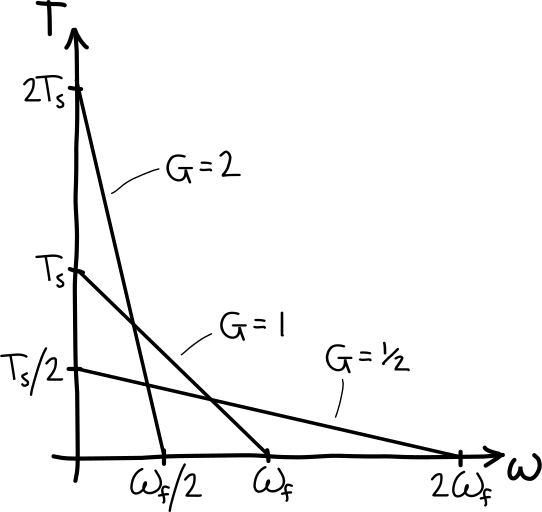
\includegraphics[width=0.4\textwidth]{Figures/GearboxCurves}\par
\end{centering}
\caption[Plot: Gearbox Torque Curves]{Gearbox torque curves. These curves are a modified version of the plots shown in \ref{fig:MotorTorqueCurveSketch}, skewed by a factor of the gearbox ratio, $G$. The greater the gearbox ratio, the greater the output torque and the smaller the output rotational speed.}
\label{fig:GearboxCurves}
\end{figure}
%

Given a specific $P_{out}, \omega, k, R, G$, and all friction = 0, we can make the plots shown in figure \ref{fig:GearboxPowerCurves}. Recall that putting on a gearbox replaces $k$ with $Gk$ and therefore


\begin{equation}
P_{in}=P_{out}+P_{out}^{2}\frac{R}{(Gk)^{2}}
\label{eq:GearboxPowerCurves}
\end{equation}


% FIGURE
\begin{figure}[]		% h="here" t="top" b="bottom" p="separate page"
\begin{centering}
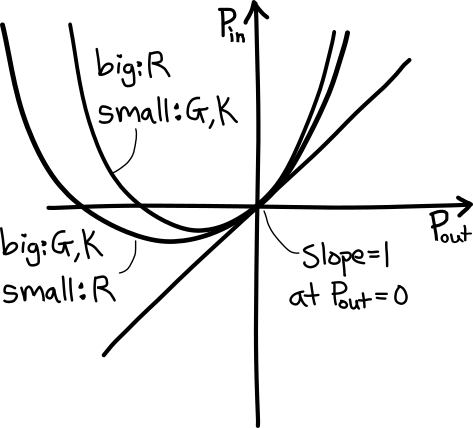
\includegraphics[width=0.4\textwidth]{Figures/GearboxPowerCurves}\par
\end{centering}
\caption[Plot: Gearbox Power Curves]{Gearbox power curves: a plot of equation \ref{eq:GearboxPowerCurves} for two relatively different values of $R$, $G$, and $k$. The curve is a parabola that intersects the origin with a slope of 1.}
\label{fig:GearboxPowerCurves}
\end{figure}
%


\section{Introduction to Muscles} % (notes page 7-9, 66)
\label{sec:IntroductionToMuscles}
\index{muscles}

Animal muscles can only work in tension. Figure \ref{fig:HumanLeg} demonstrates some terminology that is commonly used when referring to muscles. Muscles are powered by sarcomeres \index{sarcomeres}, with myosin and actin.

% FIGURE
\begin{figure}[h]		% h="here" t="top" b="bottom" p="separate page"
\begin{centering}
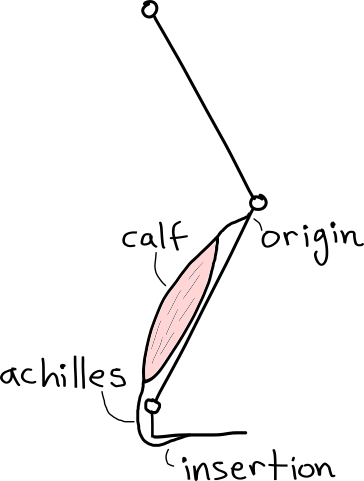
\includegraphics[width=0.3\textwidth]{Figures/HumanLeg}\par
\end{centering}
\caption[Diagram: Simple Human Leg Muscle Terminology]{Simple human leg muscle terminology. Only the calf muscle is shown, attached to bone by tendons. The origin is the point where the tendon attaches to the bone that does not move as a result of muscle contraction. The insertion is the point where the tendon attaches to the bone being actuated by the muscle. On a human leg, the calf muscle insertion tendon is called the achilles tendon.}
\label{fig:HumanLeg}
\end{figure}
%

Tendons \index{tendons} are passive connections from the muscle to the bone. The tendons are nearly perfectly elastic, though they do have a small associated hysteresis \index{tendons!hysteresis} when contracting and expanding, and are about 90 percent efficient. Tendons are very similar to springs \index{tendons!springs}, and can be modeled as such.

% FIGURE
\begin{figure}[h]		% h="here" t="top" b="bottom" p="separate page"
\begin{centering}
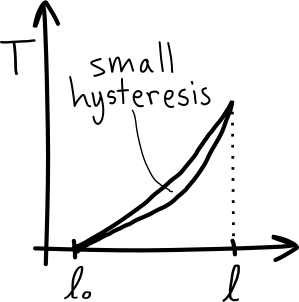
\includegraphics[width=0.3\textwidth]{Figures/TendonTensionPlot}\par
\end{centering}
\caption[Plot: Tension vs. Length for a Human Tendon]{Tension vs. Length for a human tendon. Tendons behave similarly to springs; however, there is a small hysteresis that occurs when loading and unloading tendons. The hysteresis loop forms clockwise; the tendon withstands greater force as it is being lengthened.}
\label{fig:TendonTensionPlot}
\end{figure}
%

Muscles are active motors. Up to 25\% of total fuel goes to muscle work. 50\% loss goes to metabolism in the fat to atp conversion. Another 50\% loss goes to the conversion of atp to mechanical work in the sarcomeres. Atp and calcium are what make the grab-and-release cycle happen. Calcium is the controller for the process. One part of the muscle makes atp from starch and fat, this is called metabolism.

% FIGURE
\begin{figure}[h]		% h="here" t="top" b="bottom" p="separate page"
\begin{centering}
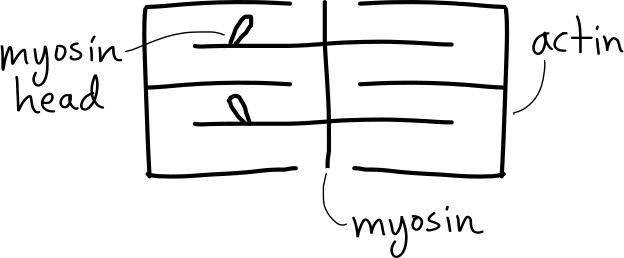
\includegraphics[width=0.45\textwidth]{Figures/Sarcomere}\par
\end{centering}
\caption[Diagram: A Sarcomere]{A sarcomere. The sarcomere is the basic functional unit responsible for muscle contraction. They are composed of myosin and actin, intertwined as shown and connected by myosin heads that act as small levers. The myosin heads connect to the actin, bend in one direction, release, and bend back to repeat the action. This motion incrementally pulls the actin closer to the myosin.}
\label{fig:Sarcomere}
\end{figure}
%

One way to measure how much energy is used during locomotion is called Indirect Calorimetry. This method measures the oxygen and carbon dioxide entering the body and leaving the body, and assumes that the intermediate chemical reaction is equivalent to burning. By measuring oxygen and carbon dioxide in this way, we can indirectly measure the amount of food that was used during locomotion. This measurement is commonly quantified by the volume of oxygen, or ``$VO_2$.'' The ratio of carbon dioxide to oxygen is telling of the ratio of starch to fat that is burned.

% FIGURE
\begin{figure}[h]		% h="here" t="top" b="bottom" p="separate page"
\begin{centering}
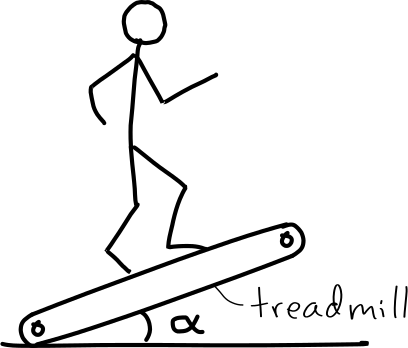
\includegraphics[width=0.35\textwidth]{Figures/Treadmill}\par
\end{centering}
\caption[Diagram: Treadmill Experiment Arrangement]{Treadmill experiment arrangement. This arrangement can be used to measure the relationship between energy use and slope of walking surface.}
\label{fig:Treadmill}
\end{figure}
%

Given a treadmill setup like the one in figure \ref{fig:Treadmill}, measurements can be made that produce a graph like the one in figure \ref{fig:MetabolicCost}.

% FIGURE
\begin{figure}[h]		% h="here" t="top" b="bottom" p="separate page"
\begin{centering}
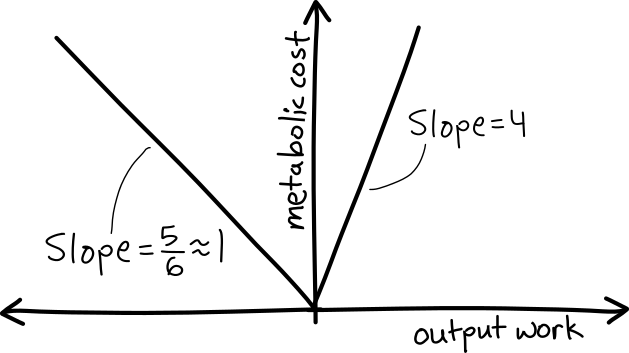
\includegraphics[width=0.5\textwidth]{Figures/MetabolicCost}\par
\end{centering}
\caption[Plot: The Metabolic Cost of Walking on a Hill]{The metabolic cost of walking on a hill. When walking on a sloped surface, the amount of output work required to move uphill increases linearly with the slope of the surface, described by the formula for potential energy, $mgh$. By experiment, it has been found that the metabolic cost of doing that work also increases linearly with slope. When walking uphill, a human uses approximately 4 times as much metabolic energy as the minimum energy required to move their mass uphill. When walking downhill, it is interesting to note that there is still a metabolic cost. A human uses approximately 5/6 as much metabolic energy as would be created if they were to roll down the hill.}
\label{fig:MetabolicCost}
\end{figure}
%

Higher slope = more tiring. Walking downhill is less tiring than walking uphill. However, it is important to note that walking downhill still consumes energy. The simplest estimate of energy cost of using muscle:

\begin{align}
P_{cost} &= C_{1}|P| \mbox{ for } P > 0\notag \\
P_{cost} &= C_{2}|P| \mbox{ for } P < 0
\label{eq:MetabolicCost}
\end{align}

where $C_{1}\approx0.25$ and $C_{2}\approx0.05$.

% FIGURE
\begin{figure}[h]		% h="here" t="top" b="bottom" p="separate page"
\begin{centering}
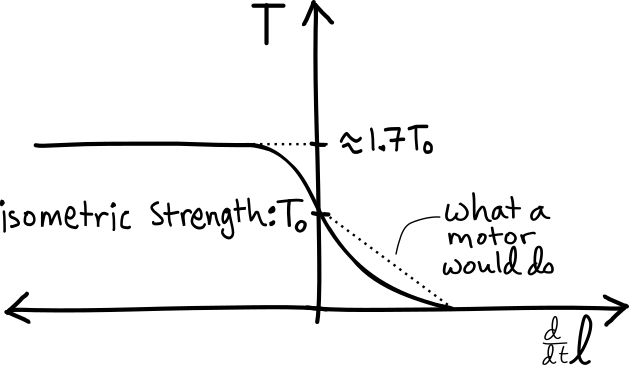
\includegraphics[width=0.5\textwidth]{Figures/LiftingVsLowering}\par
\end{centering}
\caption[Plot: Muscle Tension vs. Length Rate of Change]{Muscle tension vs. length rate of change. A muscle is capable of lowering more than it can lift. The isometric strength of a muscle $T_{0}$ describes how much force a muscle can provide with no change in length. The force a muscle can provide when lengthening is approximately 1.7 times the isometric muscle strength. A muscle in contraction provides less force the faster it contracts.}
\label{fig:LiftingVsLowering}
\end{figure}
%

Figure \ref{fig:LiftingVsLowering} says that the amount of weight that you can lower (negative work) is greater than the amount of weight that you can lift (positive work). 

% FIGURE
\begin{figure}[h]		% h="here" t="top" b="bottom" p="separate page"
\begin{centering}
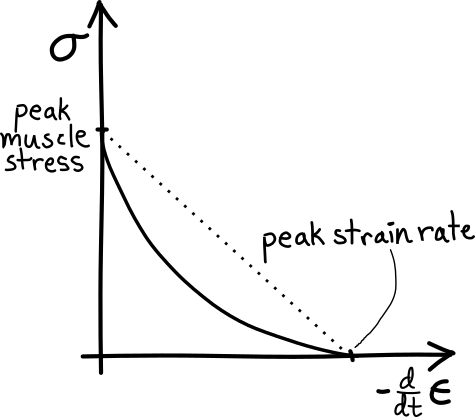
\includegraphics[width=0.4\textwidth]{Figures/PeakMuscleStress}\par
\end{centering}
\caption[Plot: Muscle Stress vs. Strain Rate]{Muscle stress vs. strain rate. The peak muscle stress can be thought of as a kind of yield strength, except instead of yielding, the muscle simply cannot hold any more and releases.}
\label{fig:PeakMuscleStress}
\end{figure}
%

Peak muscle stress is kind of like a muscle yield strength, except instead of yielding, the muscle simply cannot hold anymore and releases. For muscles, this peak muscle stress is approximately equal to 0.1\% of the yield strength of steel. 

\begin{equation}
\sigma_{peak} \approx 200 kPa
\label{eq:PeakMuscleStress1}
\end{equation}

\begin{equation}
\mbox{Peak Power} \approx \left(\frac{1}{3} \dot{\epsilon}_{peak}\right)\left(\frac{1}{3} \sigma_{peak}\right)
\label{eq:PeakMuscleStress2}
\end{equation}


\begin{equation}
\mbox{Power/Mass} \approx \frac{5[s^{-1}]}{3}\left(\frac{200000[N/m^2]}{3}\right)\frac{1}{1000[kg/m]} \approx 200 [W/kg]
\label{eq:PeakMuscleStress3}
\end{equation}

But in practice, the peak power is typically nearer to $50[W/kg]$. The best electric motors have a peak power/mass of approximately $4000[W/kg]$, but typically they are only around $200[W/kg]$. 

